\documentclass[pdftex]{beamer}
\usepackage[british]{babel}
\usepackage{graphicx}
\usepackage{url}
\usepackage[normalem]{ulem}
%\usepackage{tikz}
%\usetikzlibrary{mindmap,trees}

\mode<presentation>
\usetheme{Warsaw}
\useoutertheme{infolines}

% \usetikzlibrary{mindmap,trees,arrows,positioning}
% \tikzset{
%     %Define standard arrow tip
%     >=stealth',
%     %Define style for boxes
%     punkt/.style={
%            rectangle,
%            rounded corners,
% %           fill = purple,
%            draw=black, very thick,
%            text width=6.5em,
%            minimum height=2em,
%            text centered},
%     % Define arrow style
%     pil/.style={
% %           <->,
%            ultra thick,
%            shorten <=4pt,
%            shorten >=4pt,}
% }

\setbeamertemplate{navigation symbols}{}
% \usebeamertemplate*{logo}
% \logo{\includegraphics[height=0.85cm]{cmetlogo.png}}

% add slide number to bottom RHS (not required for infolines outer theme)
% \newcommand*\oldmacro{}%
% \let\oldmacro\insertshorttitle%
% \renewcommand*\insertshorttitle{%
%   \oldmacro\hfill%
%   \insertframenumber\,/\,\inserttotalframenumber}

\title[Digital Science Catalyst Grant]{A System for Automating Reproducibility in Science}
\author[]{Tom Crick, Benjamin A. Hall and Samin Ishtiaq}
\institute[@DrTomCrick]{\url{https://github.com/tomcrick/DSCatalyst}}
\date{17 December 2014}

\begin{document}

% titlepage
\begin{frame}
\titlepage
\end{frame}

% TOC
% \section*{Talk Outline} 
% \begin{frame} 
% \tableofcontents 
% \end{frame} 


\begin{frame}
\frametitle{Our Computational World}
%\begin{alertblock}{The future?}
{\Large{{\emph{``[Computational techniques] have moved on from assisting scientists in 
doing science, to transforming both how science is 
done and what science is done.''}}}}\\
\flushright{{\emph{Science as an open enterprise}, Royal Society (June 2012)}\\
{\scriptsize{\url{https://royalsociety.org/policy/projects/science-public-enterprise/}}}}
%\end{alertblock}
\end{frame}

\begin{frame}
\frametitle{Motivation}
\begin{center}

\includegraphics[width=0.9\paperwidth]{phd031214s.png}
\end{center}
\end{frame}

\begin{frame}
\frametitle{Motivation}
\begin{center}
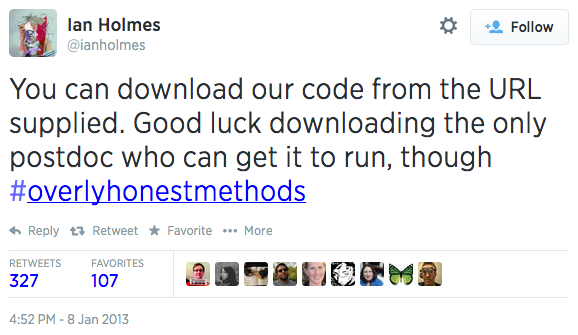
\includegraphics[width=0.9\paperwidth]{overlyhonesttweet.png}
\end{center}
\end{frame}

% { % all template changes are local to this group.
%     \setbeamertemplate{navigation symbols}{}
%     \begin{frame}[plain]
%         \begin{tikzpicture}[remember picture,overlay]
%             \node[at=(current page.center)] {
%                 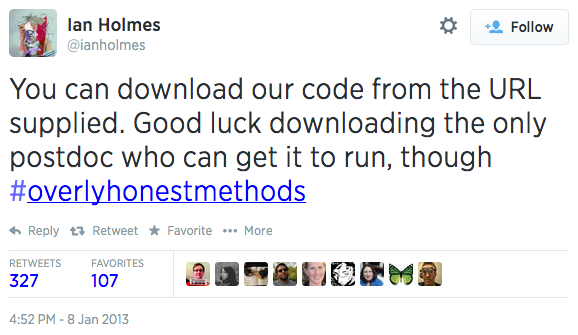
\includegraphics[width=0.9\paperwidth]{overlyhonesttweet.png}
%             };
%         \end{tikzpicture}
%      \end{frame}
% }

% { % all template changes are local to this group.
%     \setbeamertemplate{navigation symbols}{}
%     \begin{frame}[plain]
%         \begin{tikzpicture}[remember picture,overlay]
%             \node[at=(current page.center)] {
%                 
\includegraphics[width=0.9\paperwidth]{phd031214s.png}
%             };
%         \end{tikzpicture}
%      \end{frame}
% }

\begin{frame}
\frametitle{Sharing}
Two key types of results arise from work done in the computational sciences:
\begin{itemize}
\item Models
\item Algorithms
\end{itemize}
\vspace{1em}
Fundamental advantage of computer science and more broadly,
computational science: {\textbf{the unique ability to share the raw outputs of
their research as software and datafiles.}}
\end{frame}

\begin{frame}
\frametitle{A System for Automating Reproducibility in Science}
\begin{itemize}
\item Open software, algorithms and models
\item Open and community curated benchmarks
\item Integrated continuous integration system: authoritative source of results for these algorithms running on these benchmarks.
\end{itemize}
\end{frame}

\begin{frame}
\frametitle{Proposed Workflow}
\begin{center}
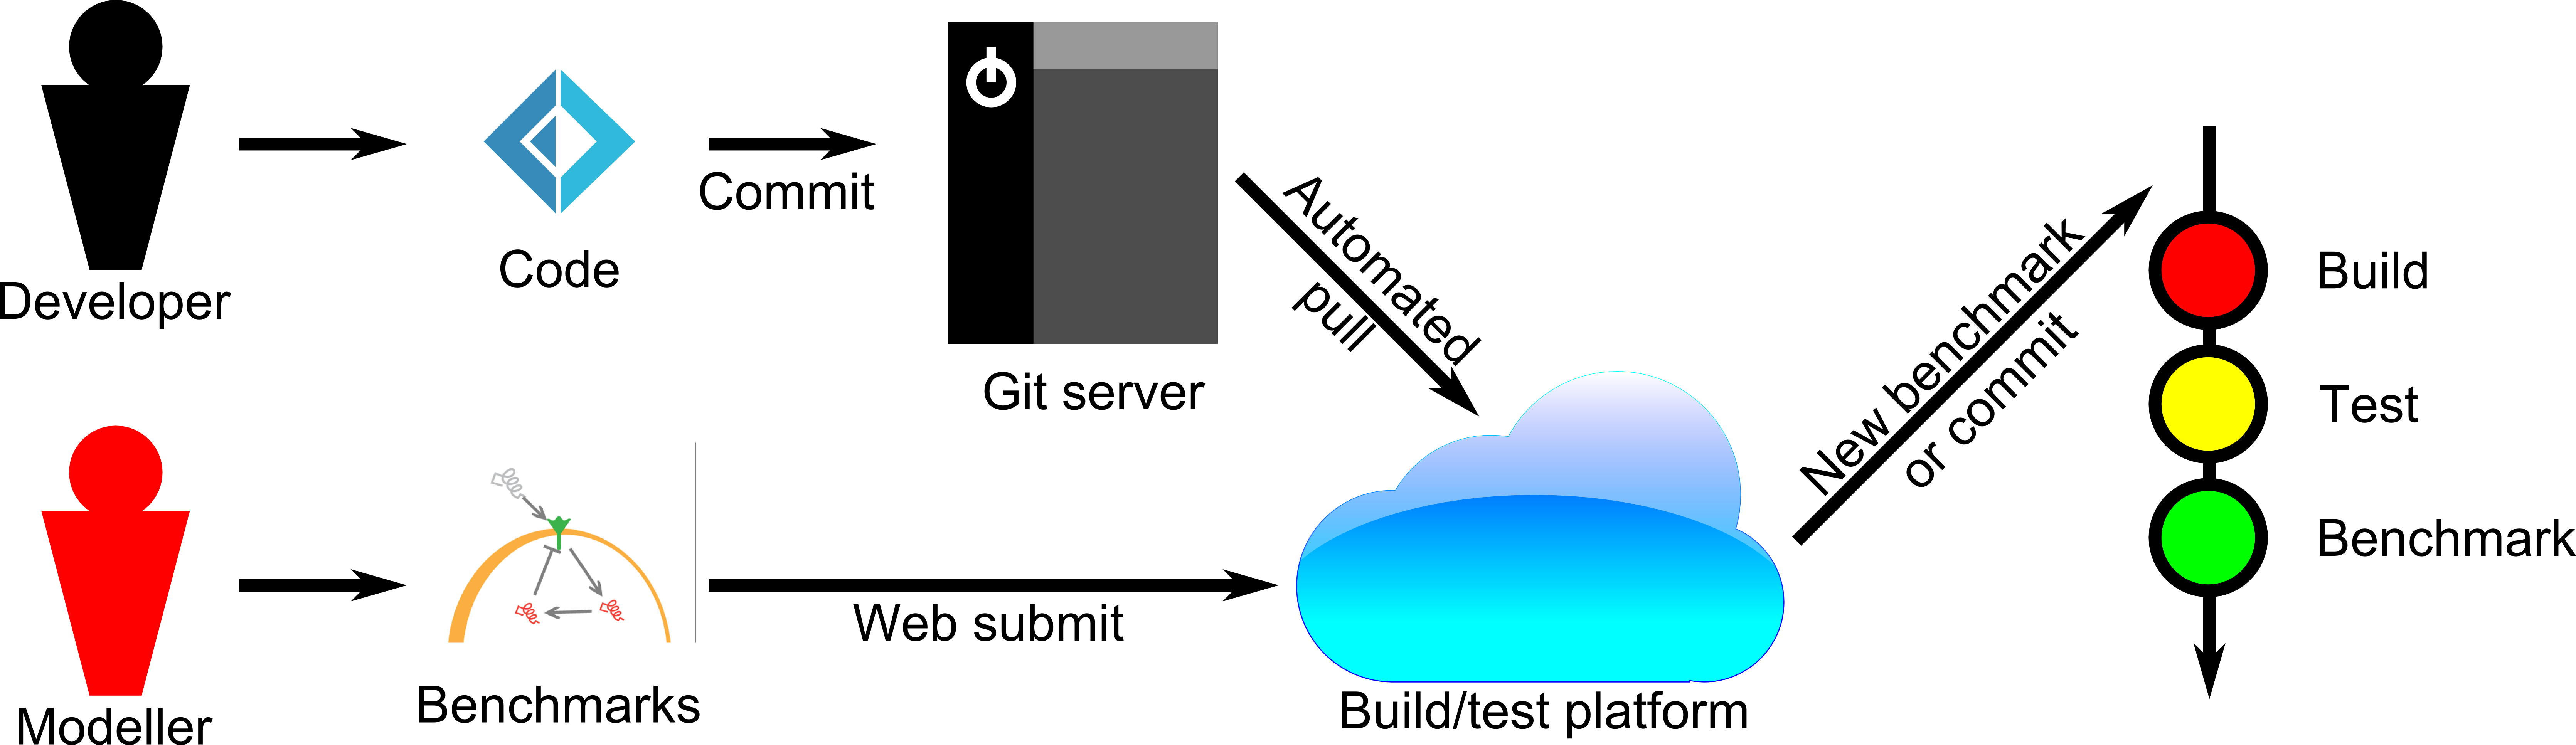
\includegraphics[width=0.9\paperwidth]{workflow.png}
\end{center}
\end{frame}

% { % all template changes are local to this group.
%     \setbeamertemplate{navigation symbols}{}
%     \begin{frame}[plain]
%         \begin{tikzpicture}[remember picture,overlay]
%             \node[at=(current page.center)] {
%                 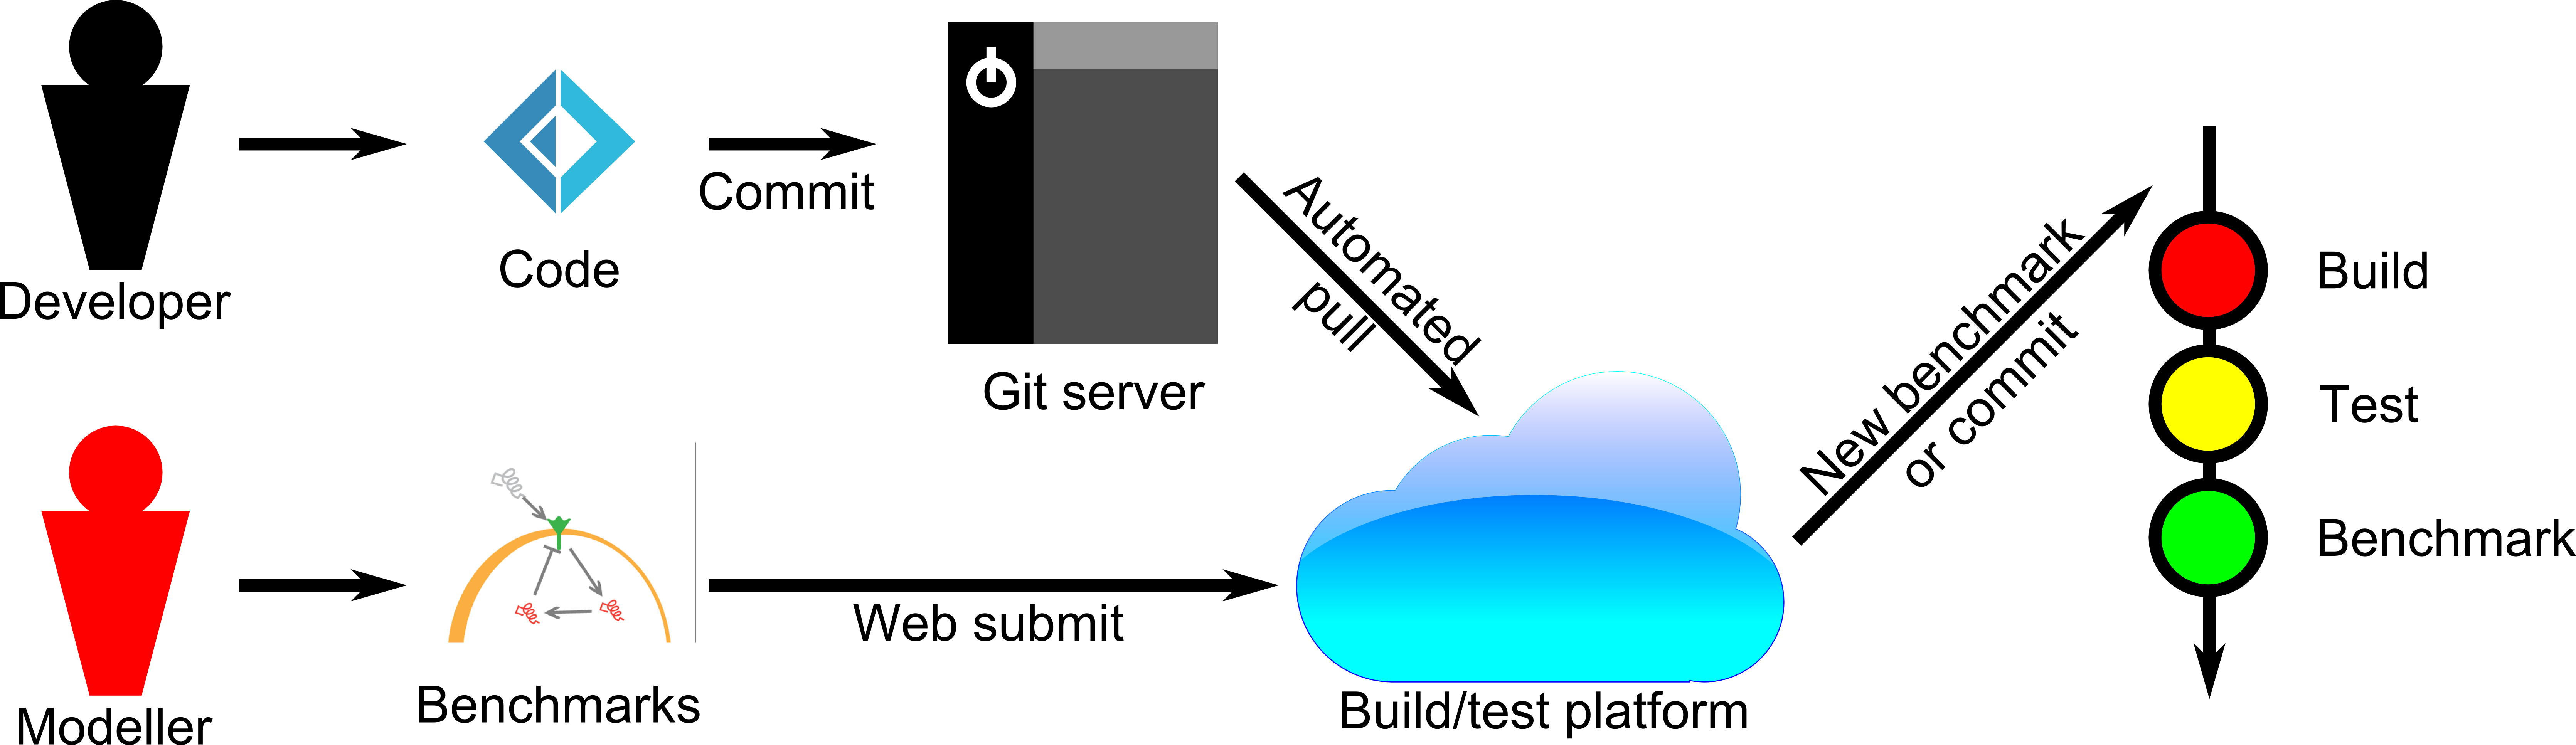
\includegraphics[width=0.9\paperwidth]{workflow.png}
%             };
%         \end{tikzpicture}
%      \end{frame}
% }


\begin{frame}
\frametitle{Plan}
{\small{\begin{itemize}
\item Build a cloud service which automatically pulls and compiles code from source repos;
\item Run automated tests defined by the developers on the code;
\item Perform analysis of benchmark sets supplied by both the developer and external users;
\item Provide persistent audit trails for software and benchmarks results;
\item Collaborate with key stakeholders in the open software/open
  data/open access/open science space, as well as key e-infrastructure
  organisations e.g. GitHub, figshare, SSI, Mozilla Science Lab,
  Digital Science, etc.
\item Follow-on funding...
\item {\textbf{Key:}} engage with communities to embed system/workflow and effect
  cultural change.
\end{itemize}}}
\end{frame}


\begin{frame}
\frametitle{References}
{\small{\begin{itemize}
\item Tom Crick, Benjamin A. Hall, Samin Ishtiaq and Kenji
  Takeda. {\emph{``Share and Enjoy'': Publishing Useful and Usable
      Scientific Models}}. In 1st International Workshop on
  Recomputability, 2014: \url{http://arxiv.org/abs/1409.0367}
\item Tom Crick, Benjamin A. Hall and Samin Ishtiaq. {\emph{``Can I Implement
  Your Algorithm?'': A Model for Reproducible Research Software}}. In
  Proceedings of 2nd International Workshop on Sustainable Software
  for Science: Practice and Experiences (WSSSPE2), 2014:
  \url{http://arxiv.org/abs/1407.5981}
\item Digital Science Catalyst Grant:
  \url{https://github.com/tomcrick/DSCatalyst} (Nov 2014)
\item Microsoft Azure for Research Grant:
  \url{https://github.com/tomcrick/Azure4Research} (Dec 2014)
\end{itemize}}}
\end{frame}

\end{document}
